\documentclass{article}

	\usepackage[english]{babel}
	\usepackage{xspace}
	\usepackage{graphicx}
	\usepackage{hyperref}

	\newcommand{\latex}{\LaTeX\xspace}
	\newcommand{\email}[1]{\texttt{#1}}

\begin{document}

\title{
	A Guide to \latex Editing in Visual Studio Code\\
	\large Written in \latex with Visual Studio Code
}
\author{
	Dan Arad\\
	\email{arda@bgu.ac.il}
}
\maketitle

\section{Introduction}
This guide's purpose is to help setup a comfortable and efficient editing of \latex documents using Visual Studio Code\footnotemark[1] (also known as VSCode). This also includes the ability to easily work with git version control, and keep generated files out of the way.\\
VSCode is a free open source powerful light-weight editor developed and maintained by Microsoft. The editor boasts many extensions and built-in git support, and is widely used. Among its many extension, there is one called \emph{LaTeX Workshop}\footnotemark[2].\\
To me VSCode is the first choice for editing any kind of code, and for that reason I chose to see how well it will preform as a \latex editor. I was not dissapointed with the result.


\section{Basic Setup}
For the basic setup of VSCode with \latex I used Nicky Marino's guide\footnotemark[3], and this entire section is based on it.\\
At the conclusion of this basic setup, you will have everything you need:
\begin{itemize}
	\item{Syntax highlighting for \latex}
	\item{Preview option that is updated either manualy, on save or on change of the document}
	\item{An outline of your \latex document}
\end{itemize}
\begin{figure}[h!]
	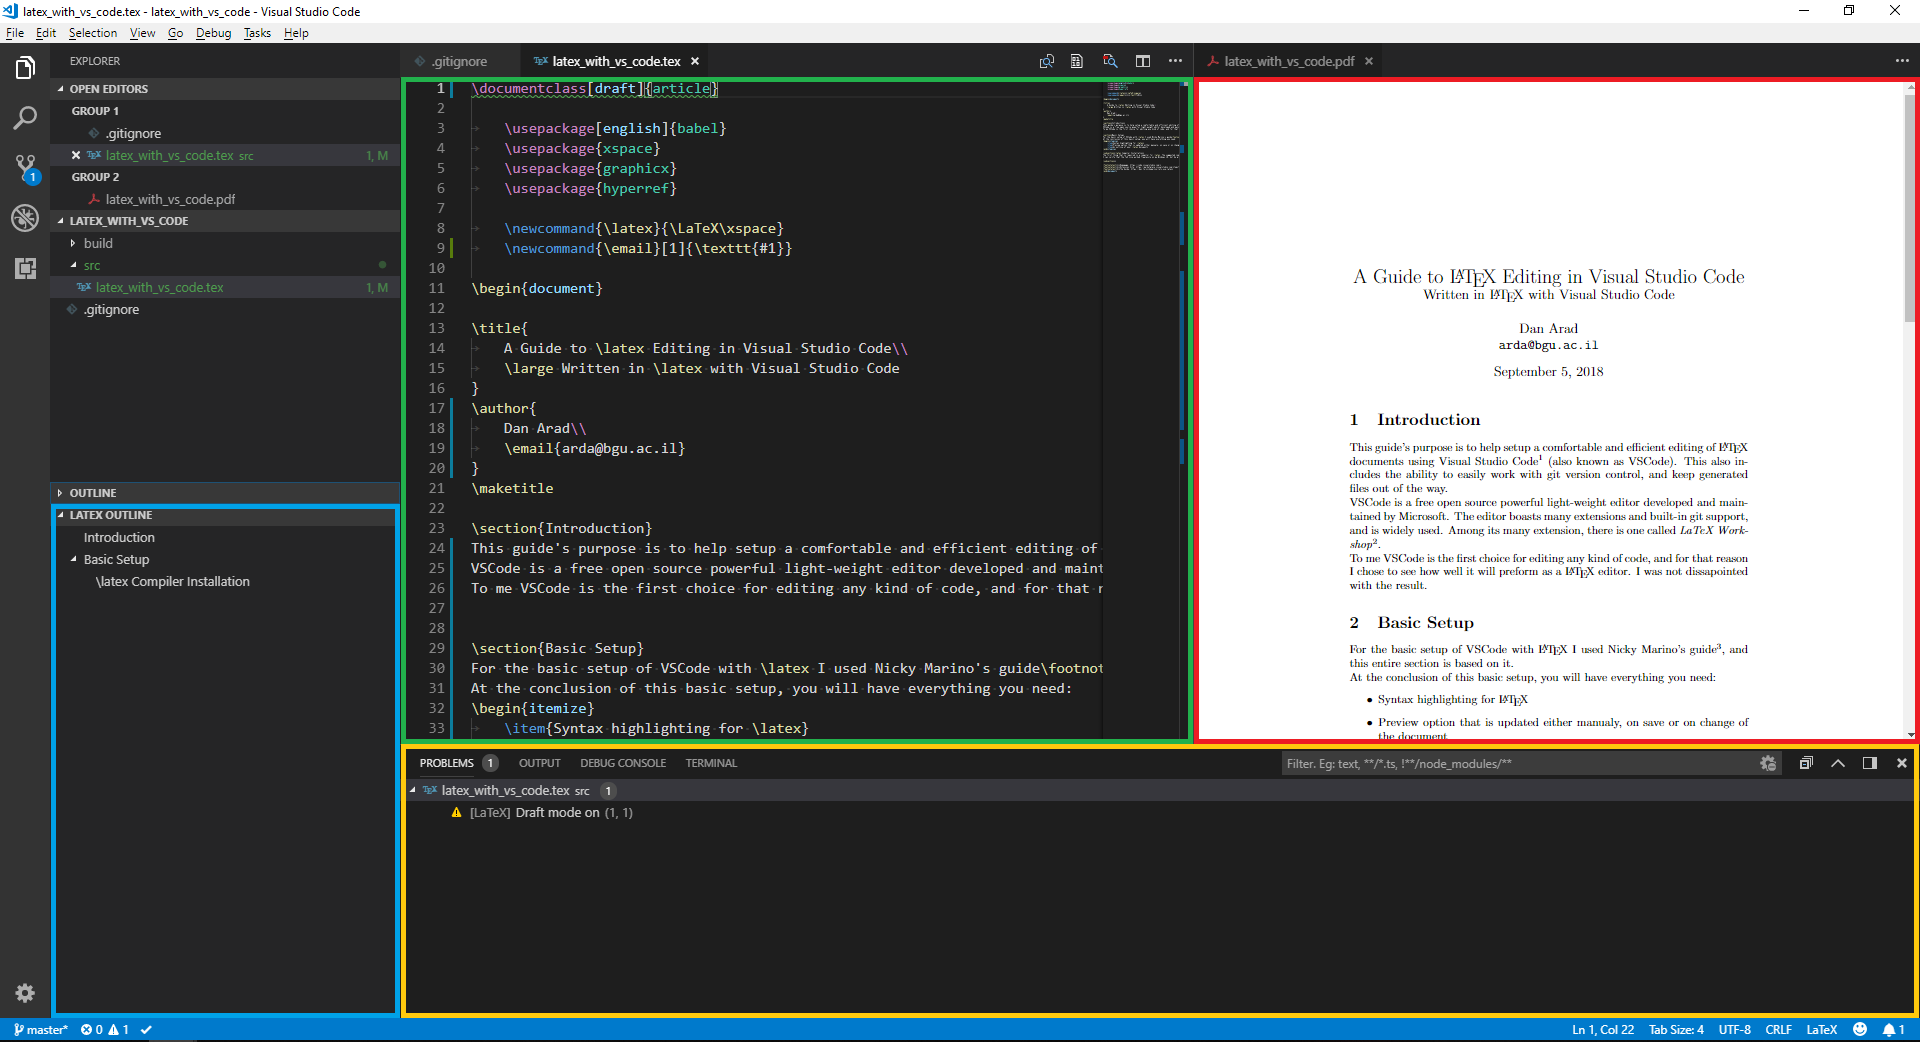
\includegraphics[width=\linewidth]{../resources/vscode_with_latex_highlights.png}
	\caption{Green: Code Highlighting, Red: Preview, Blue: Outline, Yellow: Errors and Warnings}
	\label{fig:vscode_with_latex_highlights}
\end{figure}

\subsection{\latex Compiler Installation}
The first thing that is required is a compiler for \latex. The suggested compiler is \emph{TeX Live} for Windows and Linux, and \emph{MacTex} for MacOS.\\
I can verify that the TeX Live worked flawlessly on my Windows 10, but be prepared - It's a very long installation.

\subsection{}

\footnotetext[1]{Homepage: https://code.visualstudio.com/}
\footnotetext[2]{Extension Site: https://marketplace.visualstudio.com/items?itemName=James-Yu.latex-workshop}
\footnotetext[3]{The Guide: https://dev.to/nickymarino/lets-use-latex}
\end{document}